\section{Software Architecture}
\label{sec:software-architecture}

\subsection{Module map}
\status{IMPLEMENTED}

\begin{figure}[H]
    \centering
    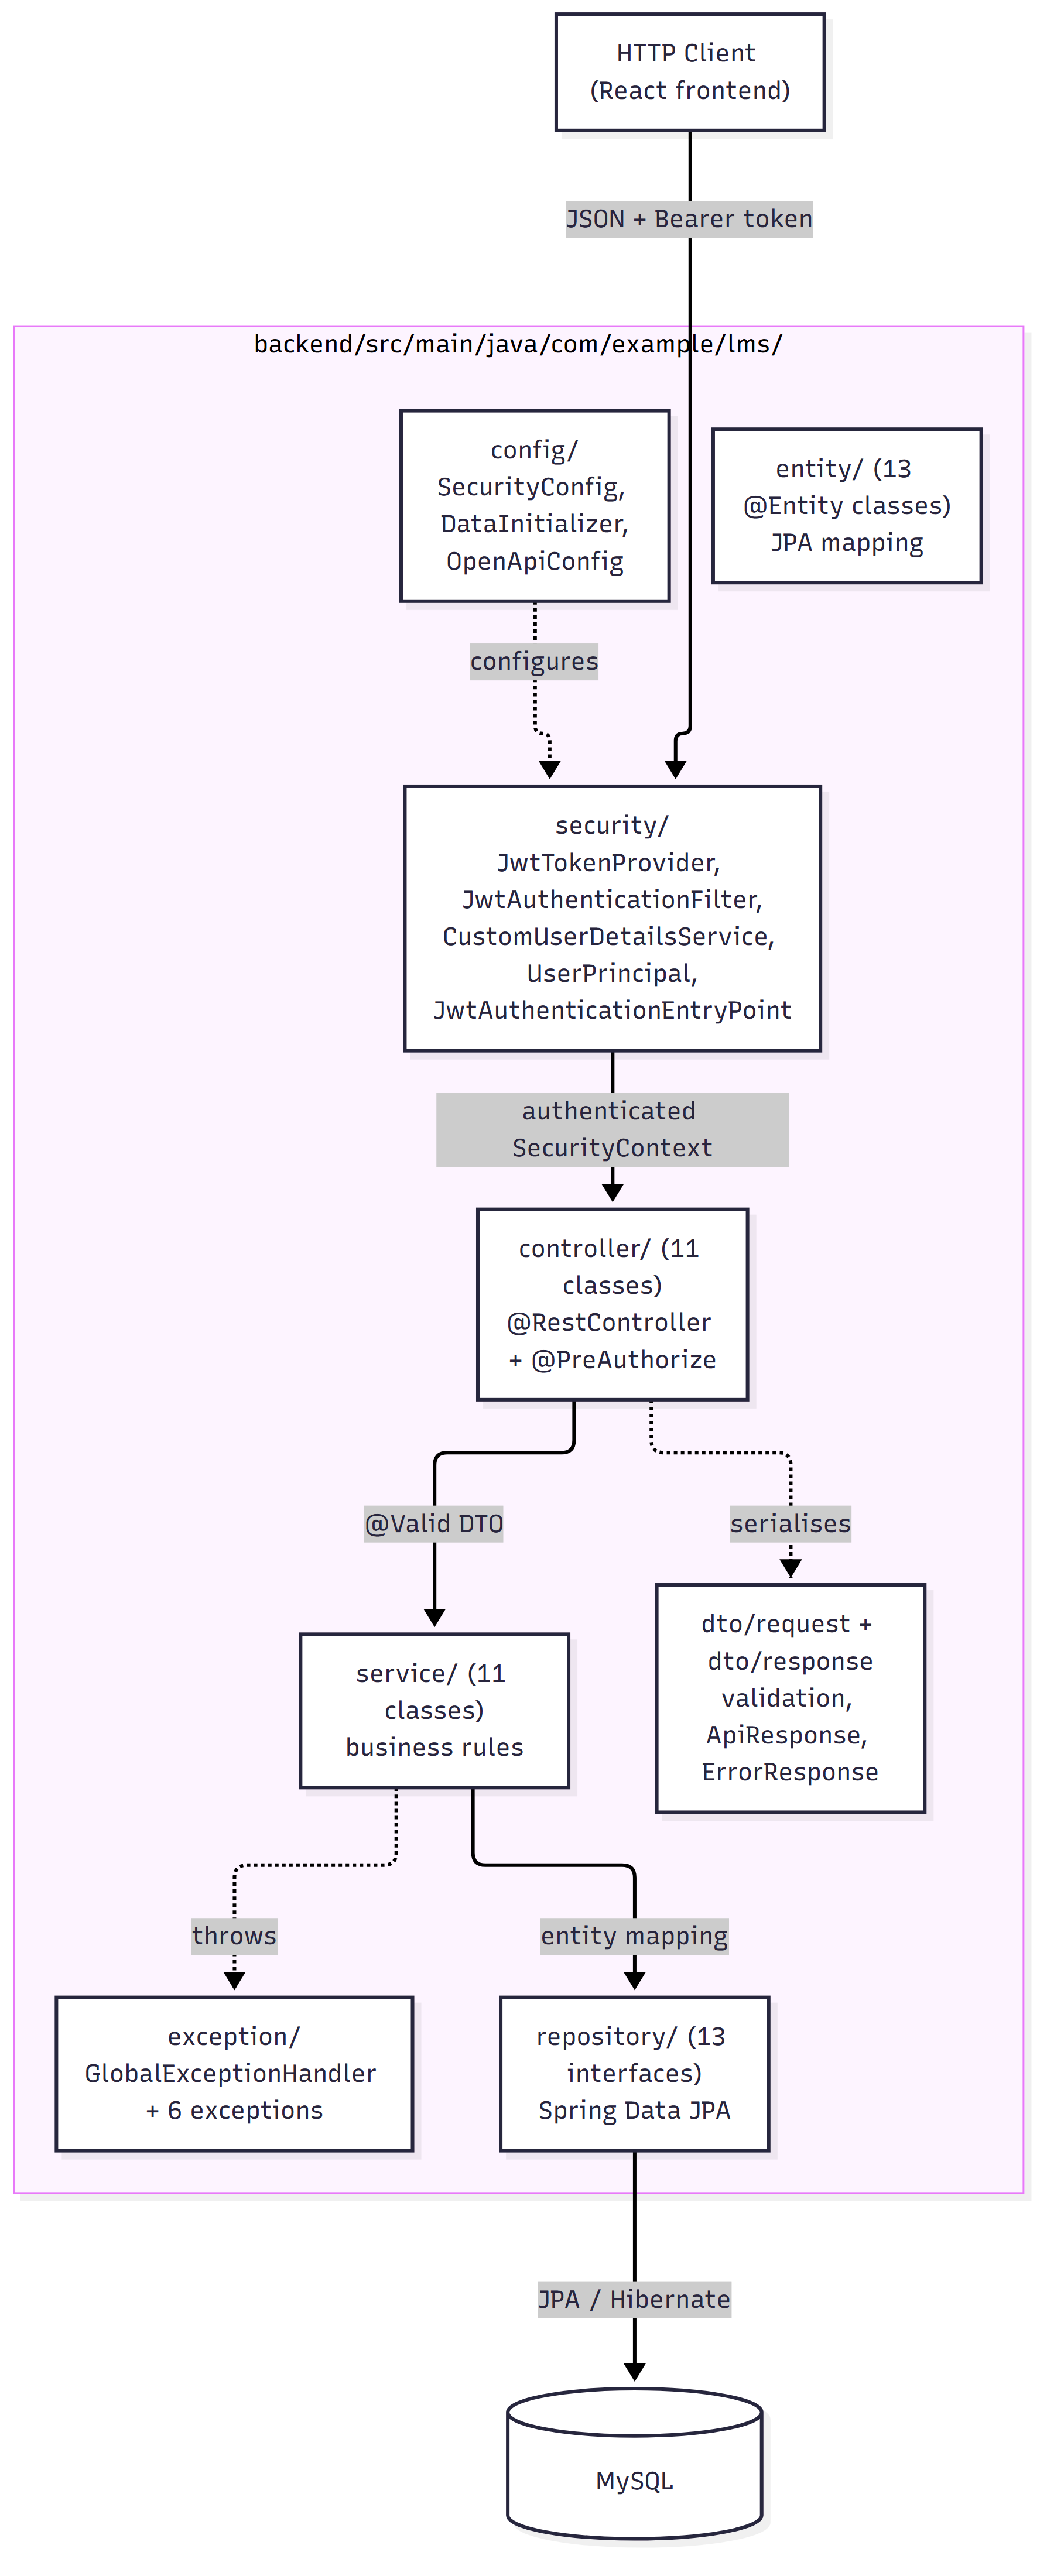
\includegraphics[width=0.92\textwidth]{diagrams/backend-layers.png}
    \caption{Backend software modules and their dependency direction}
    \label{fig:backend-layers}
\end{figure}

\begin{table}[H]
\centering
\caption{Software modules and ownership boundaries}
\label{tab:module-map}
\begin{tabular}{@{}L{4.0cm}L{5.6cm}L{4.6cm}@{}}
\toprule
\textbf{Module} & \textbf{Contents} & \textbf{Boundary rule} \\
\midrule
Frontend application & \pathref{frontend/src/} (api, components, pages, routes, context, hooks, data, utils) & Must not modify \pathref{backend/**} or \pathref{database/**} \\
Backend application & \pathref{backend/src/main/java/com/example/lms/} (8 packages) & Must not modify \pathref{frontend/**} \\
Database & \pathref{database/*.sql} & Owned exclusively by the backend workstream \\
API contract & DTO classes + \pathref{CONTRACT.md} sections 10--12 & Changes require cross-workstream agreement \\
Test suites & \pathref{backend/src/test/}, \pathref{frontend/src/test/} & Feature is incomplete until both suites pass \\
\bottomrule
\end{tabular}
\end{table}

\subsection{Backend packages (software units)}
\status{IMPLEMENTED}

\begin{table}[H]
\centering
\caption{Backend package responsibilities}
\label{tab:backend-packages}
\begin{tabular}{@{}L{2.9cm}L{6.6cm}L{4.7cm}@{}}
\toprule
\textbf{Package} & \textbf{Responsibility} & \textbf{Key classes} \\
\midrule
\code{config} & Framework wiring & SecurityConfig, DataInitializer, OpenApiConfig \\
\code{security} & Authentication pipeline & JwtTokenProvider, JwtAuthenticationFilter, CustomUserDetailsService, UserPrincipal, JwtAuthenticationEntryPoint \\
\code{controller} & HTTP adapters (11) & AuthController, CourseController, QuizController\dots \\
\code{dto} & API contracts (22 classes) & request/* + response/* \\
\code{service} & Business logic (11) & CourseService, QuizService, CertificateService\dots \\
\code{repository} & Persistence (13 interfaces) & Spring Data CRUD + derived queries \\
\code{entity} & Domain model (13) & User, Course, Lesson, Quiz, Certificate\dots \\
\code{exception} & Error taxonomy & GlobalExceptionHandler + 6 exceptions \\
\bottomrule
\end{tabular}
\end{table}

\subsection{Frontend software units}
\status{IMPLEMENTED}

\begin{table}[H]
\centering
\caption{Frontend module responsibilities}
\label{tab:frontend-modules}
\begin{tabular}{@{}L{3.2cm}L{7.0cm}L{4.0cm}@{}}
\toprule
\textbf{Module} & \textbf{Responsibility} & \textbf{Files} \\
\midrule
Entry & Bootstrap, antd theme, providers & \pathref{src/main.jsx}, \pathref{src/App.jsx} \\
Shell & Navbar, role sidebar/drawer, footer & AppShell, Navbar, Sidebar, Footer \\
Routing & Route tree + guards & \pathref{src/routes/} (AppRoutes, ProtectedRoute) \\
Pages & Screen-level composition (11 + 2 practice) & \pathref{src/pages/} \\
Components & Reusable UI (40+) & \pathref{src/components/} incl. practice/ and ui/ \\
API layer & 11 feature modules + shared client & \pathref{src/api/} \\
Auth state & Session context, role derivation & \pathref{src/context/AuthContext.jsx} \\
Practice data & Static problem dataset (swap boundary) & \pathref{src/data/practiceData.js} \\
Utilities & Constants, formatters & \pathref{src/utils/} \\
Tests & Vitest suites (8 files) & \pathref{src/test/} \\
\bottomrule
\end{tabular}
\end{table}

\subsection{Component interaction}
\status{IMPLEMENTED}

\begin{figure}[H]
    \centering
    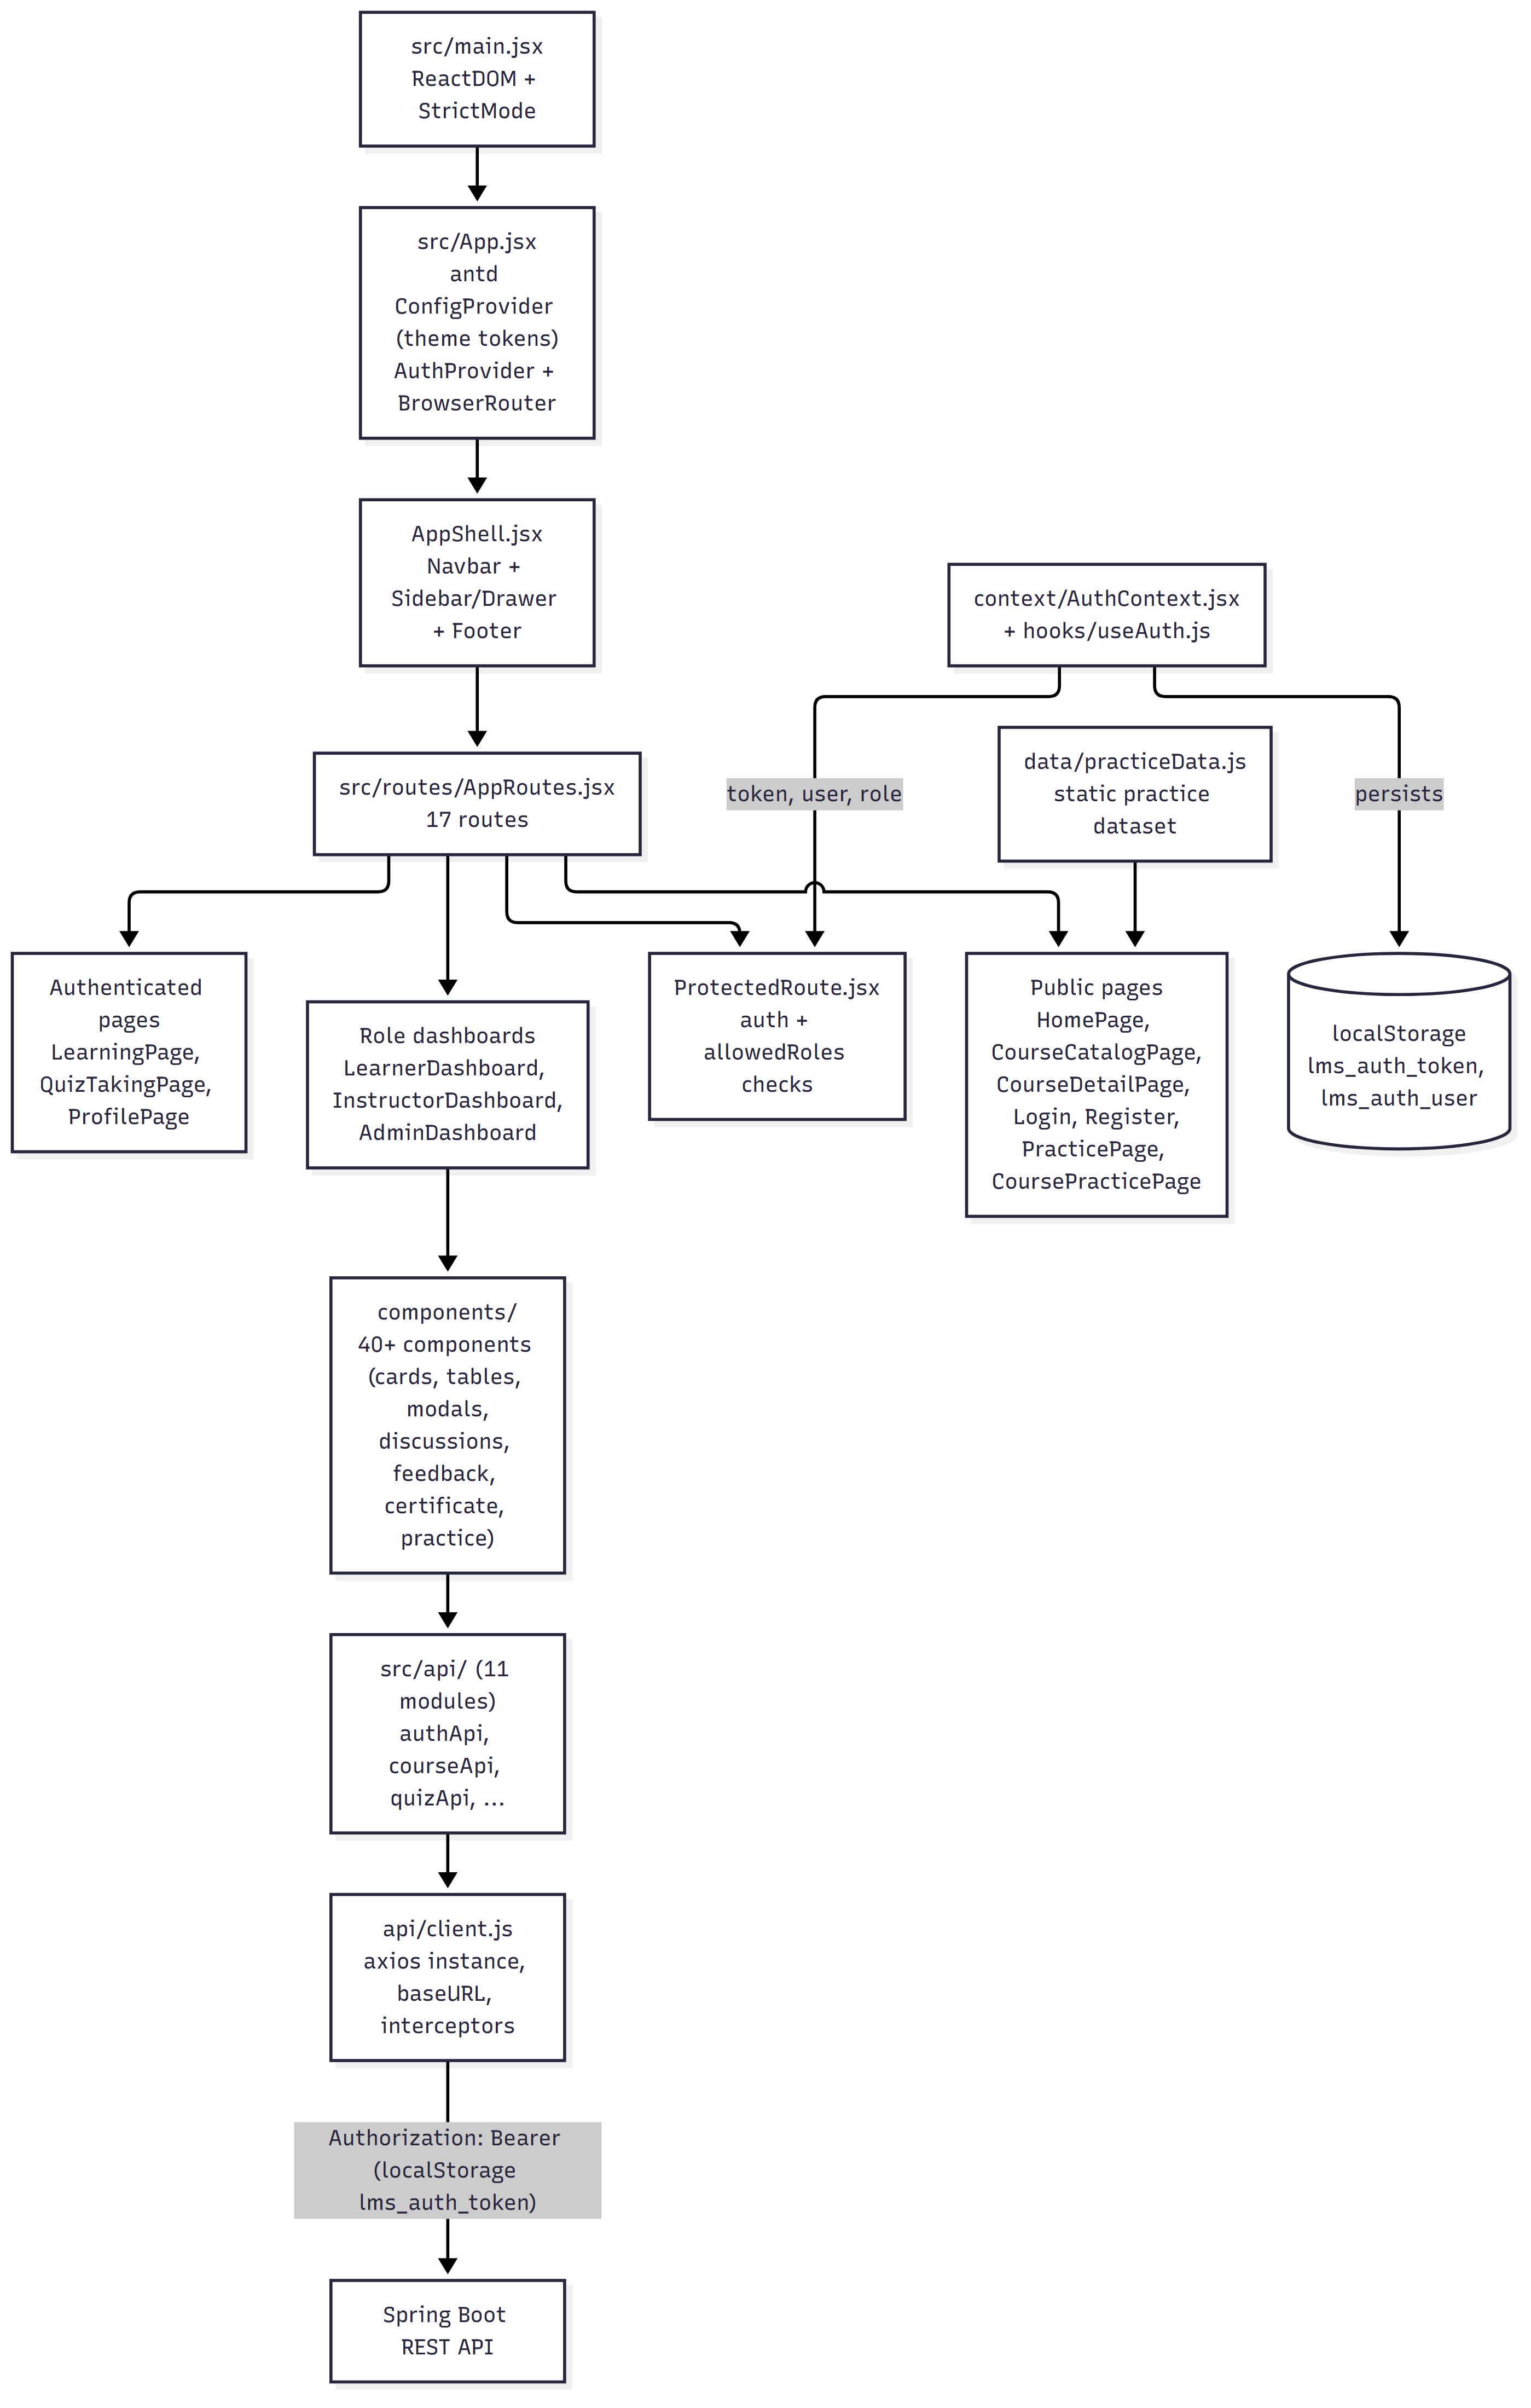
\includegraphics[width=0.95\textwidth]{diagrams/frontend-architecture.png}
    \caption{Frontend component architecture and data flow to the API}
    \label{fig:frontend-arch}
\end{figure}

\subsection{Data ownership and consistency}
\status{IMPLEMENTED}

\begin{itemize}
    \item MySQL is the single source of truth for users, catalogue, enrolments, progress, attempts, discussions, feedback and certificates.
    \item The backend owns all writes; the client may only send intentions (e.g.\ \code{{completed: true}}), never authoritative results (scores, eligibility).
    \item Transactions: service methods are \code{@Transactional} where multi-write (e.g.\ \code{AuthService.register}); each HTTP request is a single logical unit of work.
    \item Optimistic concurrency control (version columns) is \status{NOT IMPLEMENTED} -- concurrent updates last-write-wins.
\end{itemize}

\subsection{Cross-cutting concerns}
\begin{table}[H]
\centering
\caption{Cross-cutting concerns and their implementation points}
\label{tab:crosscutting}
\begin{tabular}{@{}L{3.4cm}L{6.2cm}L{4.6cm}@{}}
\toprule
\textbf{Concern} & \textbf{Mechanism} & \textbf{Location} \\
\midrule
Authentication & JWT filter before \code{UsernamePasswordAuthenticationFilter} & \pathref{security/JwtAuthenticationFilter.java} \\
Authorisation & URL rules + \code{@PreAuthorize} + service ownership checks & SecurityConfig, controllers, services \\
Validation & Bean Validation on DTOs & \code{dto/request/*} \\
Error handling & \code{@RestControllerAdvice} mapping to envelopes & \pathref{exception/GlobalExceptionHandler.java} \\
Logging & SLF4J with package log levels & \code{application.yml} \\
API docs & springdoc annotation-driven OpenAPI & \pathref{config/OpenApiConfig.java} \\
Client errors & Axios interceptor maps backend error codes & \pathref{frontend/src/api/client.js} \\
UI states & Loading/Error/Empty primitives & \pathref{frontend/src/components/common/} \\
\bottomrule
\end{tabular}
\end{table}
